\begin{figure}[htbp]
    \centering

    % Top panel for the image
    \begin{subfigure}[b]{\textwidth}
        \centering
        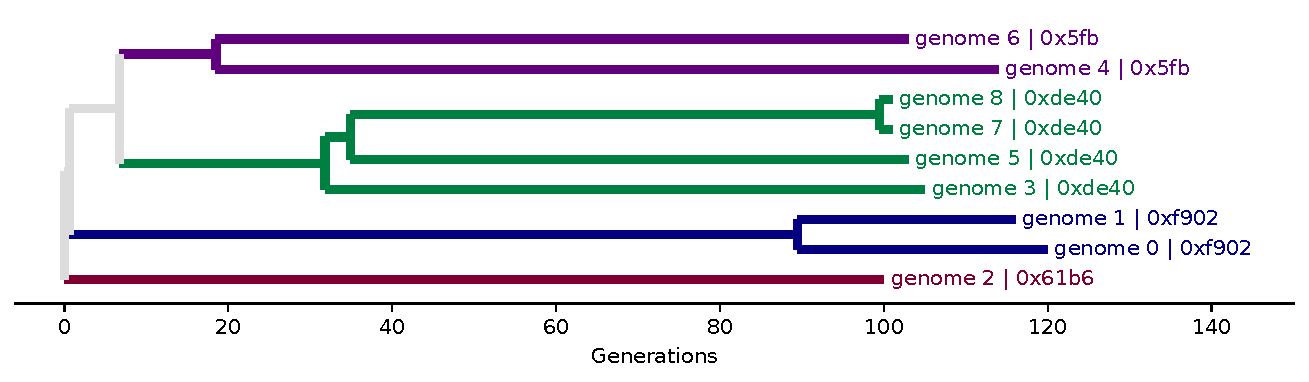
\includegraphics[width=0.7\textwidth]{binder/binder/teeplots/genome=hsurftiltedsticky_tagged+viz=draw-biopython-tree+ext=}
        \caption{%
          Reconstructed phylogeny, generated under the assumption of shared ancestry.
          Hexidecimal codes in taxon names are fixed random markers generated at simulation start-up, indicating independent lineage originations.
          Color coding indicates clades with independent lineage originations.
          As expected, low relatedness is predicted for taxa originating from independent lineages.
        } \label{fig:validation-example:phylogeny}
    \end{subfigure}

    % Space between image and table
    \vspace{10pt}

    % Bottom panel for the table
    \begin{subfigure}[b]{\textwidth}

\begin{minipage}[t]{\textwidth}
\centering
\footnotesize
\begin{tabular}{
c
>{\columncolor{LighterBlue}}c
>{\columncolor{LighterBlue}}c
>{\columncolor{LighterSalmon}}c
>{\columncolor{LighterSalmon}}c
q % Thick divider
>{\columncolor{LighterPastelGreenYellow}}c
>{\columncolor{LighterPastelGreenYellow}}c
>{\columncolor{LighterPastelGreenYellow}}c
>{\columncolor{LighterPastelGreenYellow}}c
q % Thick divider
>{\columncolor{LighterPastelGreenYellow}}c
>{\columncolor{LighterPastelGreenYellow}}c
>{\columncolor{LighterPastelGreenYellow}}c
>{\columncolor{LighterPastelGreenYellow}}c
}
& \multicolumn{4}{cq}{\cellcolor{white}Word 0} & \multicolumn{4}{cq}{\cellcolor{white}Word 1} & \multicolumn{4}{c}{\cellcolor{white}Word 2} \\
\cmidrule(l{1.5pt}r{1.5pt}){2-5}
\cmidrule(l{1.5pt}r{1.5pt}){6-9}
\cmidrule(l{1.5pt}r{1.5pt}){10-13}
Byte & {\cellcolor{white}0} & {\cellcolor{white}1} & {\cellcolor{white}2} & {\cellcolor{white}3} & {\cellcolor{white}4} & {\cellcolor{white}5} & {\cellcolor{white}6} & {\cellcolor{white}7} & {\cellcolor{white}8} & {\cellcolor{white}9} & {\cellcolor{white}10} & {\cellcolor{white}11} \\
\cmidrule(l{1.5pt}r{1.5pt}){2-2}
\cmidrule(l{1.5pt}r{1.5pt}){3-3}
\cmidrule(l{1.5pt}r{1.5pt}){4-4}
\cmidrule(l{1.5pt}r{1.5pt}){5-5}
\cmidrule(l{1.5pt}r{1.5pt}){6-6}
\cmidrule(l{1.5pt}r{1.5pt}){7-7}
\cmidrule(l{1.5pt}r{1.5pt}){8-8}
\cmidrule(l{1.5pt}r{1.5pt}){9-9}
\cmidrule(l{1.5pt}r{1.5pt}){10-10}
\cmidrule(l{1.5pt}r{1.5pt}){11-11}
\cmidrule(l{1.5pt}r{1.5pt}){12-12}
\cmidrule(l{1.5pt}r{1.5pt}){13-13}
& \multicolumn{4}{cq}{\cellcolor{white}} & \multicolumn{4}{cq}{\cellcolor{white}} & \multicolumn{4}{c}{\cellcolor{white}} \\[-2ex]
\scriptsize{Genome 0} & \texttt{F9} & \texttt{02} & \texttt{79} & \texttt{00} & \texttt{8D} & \texttt{22} & \texttt{4F} & \texttt{F3} & \texttt{D2} & \texttt{78} & \texttt{AD} & \texttt{C7} \\
& \multicolumn{4}{cq}{\cellcolor{white}} & \multicolumn{4}{cq}{\cellcolor{white}} & \multicolumn{4}{c}{\cellcolor{white}} \\[-2ex]
\scriptsize{Genome 1} & \texttt{F9} & \texttt{02} & \texttt{75} & \texttt{00} & \texttt{8D} & \texttt{A1} & \texttt{CB} & \texttt{F2} & \texttt{D1} & \texttt{5B} & \texttt{CC} & \texttt{D4} \\
& \multicolumn{4}{cq}{\cellcolor{white}} & \multicolumn{4}{cq}{\cellcolor{white}} & \multicolumn{4}{c}{\cellcolor{white}} \\[-2ex]
\scriptsize{Genome 2} & \texttt{61} & \texttt{B6} & \texttt{65} & \texttt{00} & \texttt{66} & \texttt{29} & \texttt{B4} & \texttt{F0} & \texttt{62} & \texttt{99} & \texttt{5A} & \texttt{61} \\
{\cellcolor{white}\ldots} & {\cellcolor{white}\ldots} & {\cellcolor{white}\ldots} & {\cellcolor{white}\ldots} & {\cellcolor{white}\ldots} & {\cellcolor{white}\ldots} & {\cellcolor{white}\ldots} & {\cellcolor{white}\ldots} & {\cellcolor{white}\ldots} & {\cellcolor{white}\ldots} & {\cellcolor{white}\ldots} &
{\cellcolor{white}\ldots} & {\cellcolor{white}\ldots} \\
\end{tabular}
\end{minipage}


        \caption{%
          Example genomes sampled after simulation completion.
          In validation testing, genomes were composed of three 32-bit words.
          The first two bytes (blue) are fixed random markers generated at simulation start-up, indicating independent lineage originations.
          The next two bytes (salmon) are a generation counter.
          Bits within the final eight bytes are lineage checkpoint values to facilitate phylogenetic reconstruction, arranged according to a tilted hereditary stratigraphic algorithm.
          Note that this genome does not include any content affecting agent traits or fitness --- neutral selection was used for this validation experiment.
        } \label{fig:validation-example:genomes}
    \end{subfigure}

    \caption{
      Synopsis of preliminary experiment used to validate Cerebras Software Language implementation of asynchronous agent-based evolution framework and hereditary stratigraphy algorithms.
      Experiments were performed on Cerebras SDK hardware simulator.
      Subfigure \ref{fig:validation-example:phylogeny} shows an example reconstructed phylogeny from genomes tagged with fixed random identifiers that identify independent lineage originations.
      Subfigure \ref{fig:validation-example:genomes} overviews layout of fixed-size genomes used for validation testing and shows example end-state genomes corresponding to phylogeny taxa.
    }
    \label{fig:validation-example}
\end{figure}
